\documentclass[runningheads]{llncs}

%PACKAGES
\usepackage[utf8]{inputenc}
\usepackage{listings, xcolor}
\usepackage{graphicx} 
\usepackage{lipsum}
\usepackage{float}
\usepackage{listings-rust}
\setcounter{secnumdepth}{5}
\begin{document}
\title{Comparing FreeST, Go and Rust}
\author{Jorge Martins\inst{1} \and
Diogo Lopes\inst{1}
}
\definecolor{darkblue}{rgb}{0.0, 0.0, 0.55}
\lstset{language=Java,
numbers=none,
keywordstyle = \color{blue},
commentstyle = \color{darkblue},
breaklines = true,
showstringspaces = false,
tabsize = 4,
basicstyle=\small,
} 
\institute{Departamento de Informática da Faculdade de Ciências da Universidade de Lisboa
\email{\{fc51033,fc51058\}@alunos.fc.ul.pt}}
\nocite{*}
\maketitle
\thispagestyle{empty}
\begin{abstract}
FreeST is an experimental functional programming language being developed at LASIGE that offers primitives to thread creation and channel communication, different to those in programming languages such as Go and Rust, that are currently being appraised by their performance and reliability. Despite being different, these languages can be compared by the characteristics of their common primitives and by their learning curve. Although there are several articles comparing Rust and Go, they mainly focus in performance and reliability instead of the learning curve of each language and their approach to channel communication and thread creation. FreeST on the other hand, due to the small community working on it, is yet to be compared to the others.
In order to compare the three languages we used an algorithm that focuses on thread creation, communication using channels and thread synchronization using those same channels. To implement this algorithm we learned the three languages so that we could comment on the difficulties and different aspects of each.
This comparison is useful to understand what aspects of some languages could benefit the others and also to inform about what difficulties developers may find when writing code in each of them.
\keywords{FreeST \and Rust \and Go.}
\end{abstract}
\section{Introduction}
Rust and Go are languages that are growing in popularity due to their performance and reliability, according to the TIOBE index, and FreeST\cite{freest} on the other hand is a very recent programming language that is still being developed at LASIGE, a research center in the Faculty of Sciences of the University of Lisbon. 
In order to compare these three languages, that were completely new to each of us until the start of this project, we aimed to understand the basic concepts of each one, such as the ownership and lifetimes in Rust or the session types \cite{session} in FreeST.

When starting to learn a new language we need to understand how the basics of that language work, and therefore our initial focus was to learn those basic concepts in each language. Once we had a clear view of this concepts we focused on the concurrency primitives of these programming languages since in this project we mainly aimed to show the differences between how each one of them handles concurrency and channels communication.

To see this differences in action we used a simple algorithm simulating a communication between a customer and a travel agency that would eventually spawn a service to finish a transaction. This way, we could see in action the creation of threads, since each of these entities will run in a different thread. This algorithm also allows to see how channel communication functions in each programming language because these threads use channels as a form of communication. Finally we can see how these channels can offer thread synchronization as well.

Our goal was to implement this algorithm in Rust, Go and FreeST, in order to understand the main differences and characteristics of each language and identifying the main complications we had while learning them.
\section{Background}
\subsection{The Plane Ticket Algorithm}
\label{alg}
In order to explore the interprocess communication through channels and thread creation, we used a simple algorithm that simulates a customer trying to buy a plane ticket from an agency, that can eventually create a service to finish the transaction with the customer. The customer, the agency and the service will be executed in different threads and will communicate through rendezvous channels, meaning that sends and receives block until the message is passed.
\begin{figure}[H]
\centering
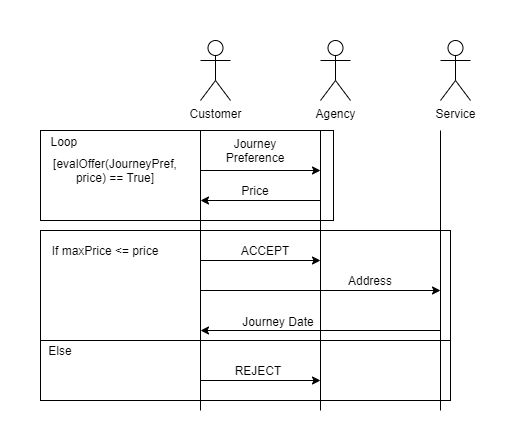
\includegraphics[scale=0.4]{Algorithm.png}
\caption{Plane Ticket Algorithm System Sequence Diagram}
\label{ssd}
\end{figure}
As we can see in figure \ref{ssd}, the algorithm consists in an early stage of negotiation where a customer will send a journey preference(e.g. "Rome") to the agency and receive the price for a ticket to the given preference repeatedly until evalOffer evaluates to true.
At this point the customer will make a choice:
\begin{itemize}
\item If the received price is lower or equal to the max accepted price of the customer, he will accept the offer.
The agency will spawn a service which will receive the customer address and send the journey date.
\item If the received price is greater than the max accepted price of the customer, he will reject the offer and end the communication.
\end{itemize}
\subsection{Rust}
Rust is a programming language that greatly focuses in performance, concurrency safety and memory management.
It introduces many core features such as ownership, lifetimes and the absence of garbage collection.
Ownership is usually a new concept for programmers that is built over three simple rules:
\begin{itemize}
\item Each value in Rust has a variable that’s called its owner;
\item There can only be one owner at a time;
\item When the owner goes out of scope, the value will be dropped.
\end{itemize}

The most important rule is the 3rd. Once the lifetime of the owner of a value ends, that value is dropped in memory. This is a key aspect of the memory management model of Rust because this way we don't need to have a garbage collector like Java has, that is constantly checking if a value can be erased from memory and by doing so it has a negative impact on the performance of a program. With ownership, Rust as no need for a garbage collector and therefore its performance is greatly enhanced, being on par with languages like C and C++. Therefore, with ownership once we move a variable to a function(as an argument) it stops being available to the function it was currently in.

Another concept that we don't usually see in other programming languages is marking a variable as mutable or immutable in its assignment. By default a variable is immutable and therefore we can't change it afterwards, meaning we must explicitly mark a variable as mutable in order to change it later in the program.

Finally, unlike what we will see in Go and FreeST, Rust does not have primitives to create threads or channels. Therefore, to do so we need to import crates that support thread creation and channels creation.
\subsection{Go}
Go is a programming language designed at Google that focuses in performance, usability and multiprocessing.
It is statically typed, meaning it checks the type safety of the program by analysing the source code. Therefore we know at compilation time what errors we might have committed.

It introduces a new primitive called Goroutines, a form of lightweight threads, meaning they share context with other goroutines in a program. They are also managed by the Go runtime, that will be responsible for the scheduling of each goroutine. This means that if one goroutine is blocked, Go's run-time will switch to another with work to do.
Goroutines run over a set of threads that by default match the number of logical processors of the environment. Of course this can be changed with the {\it GOMAXPROCS} function that sets the number of logical processors that the go program can access. Another great aspect of goroutines is that they achieve all this with a very small overhead in memory, allowing the execution of a great number of them.

Go treats channels as first class objects, in contrast with most of the other languages that offer them through external packages, or crates as we will see in Rust. This channels allow goroutines to communicate between themselves and it also allows to synchronize this same goroutines, because the channels block until the sender/receiver are ready to continue.

Go was also built to be simple to understand, and because of that its syntax is very easy to learn. We can observe this in goroutines that can be started with a simple "{\it go func()}" or the channels, constructed with "{\it c := make(chan string)}"
This language also encourages developers to write good code, emitting warnings to bad practices such as unused variables or unused imports, keeping the code clean.
\subsection{FreeST}
FreeST is a programming language developed at LASIGE, that focuses on thread creation and channel communication. Its syntax is very similar to Haskell and it introduces a very powerful tool: context-free session types based channels.

Session types describe communications in heterogeneous channels with a tail recursive structure\cite{session}.
For example we can describe a channel that sends a String and receives an Int in a very simple way
\begin{lstlisting}[language=haskell]
type exampleC : SL = !String;?Int
\end{lstlisting}
This allows a programmer to send different types in a channel without having to wrap it in a new type structure.
It also allows to use {\it Choices}, in order for the thread to choose which communication path it will follow:
\begin{lstlisting}[language=haskell]
type exampleC : SL = +{ChoiceOne: !String;?Int, ChoiceTwo: !String;?String}
\end{lstlisting}
This is achieved by the select keyword that, as the name indicates, selects the desired branch. The other end of the communication will then learn which choice was made by matching the channel with one of the many choices it is allowed to make.
The {\it send} and {\it receive} functions send a message through a given channel and receive a message from a given channel, respectively, returning, in the end, whatever is left for that channel to do.

Another concept to have in mind when using FreeST is the notion of Kind, that divides types into 4 categories:
functional(T), session(S), linear(L) and unrestricted(U).
The channels we mentioned above are of type SL, meaning they are linear session types. This means they must be fully consumed once created, or otherwise the compiler will emit an error.
Similar to Go and Rust these channel are blocking, allowing us to synchronize the threads by simply waiting for and sending messages.
\section{Implementation Details}
\subsection{Rust}
In Rust we start by defining some mock values for the max price, journey preference and customer address. It then spawns the thread that will be executing the customer's side algorithm and, at the end, it joins this thread so that the main function won't end before the transaction ends(similar to the purpose of the {\it WaitGroup} in Go and the !Bool channel in FreeST). Main is also responsible for creating a channel for the communications. We started by using the channels offered by the {\bf mpsc} crate but these channels are for, as the name of the crate indicates, multiple producers and one consumers, which is not the case of our algorithm. This being said we opted to use channels from the {\bf chan} crate, where we could freely clone any side of the channel(send side and receiver side) which was very useful due the ownership concept(we had to clone the channel because if we pass it to the other thread it will stop being available to the current).

When creating a channel we need to indicate the type of the values it will pass. Since the type vary along the plane ticket algorithm we implemented a {\it Enum} that enumerated all the possible message types. The channel was constructed over this enum type. Enums are a very powerful tool since each field in an enum can be implemented in order to receive parameters(e.g. {\it Message::JourneyPreference(jpref}). Of course, this means  that every time a message is received we need to match it to the available types, making sure we did not receive something that we shouldn't have.

The algorithm then proceeds as mentioned in section \ref{alg}. The customer thread spawns the agency thread, passing it clones of both ends of the channel. They exchange journey preferences and prices until the customer {\it evalOffer}(returning true if a random number is even) evaluates to true. The customer then decides to "ACCEPT" or "REJECT" the offer, according to his pre established max price. If rejected the transaction ends. If accepted the agency will spawn the service thread and pass it the cloned channel. This way the customer can send the address to the service and receive a randomly generated date from it, thus ending the transaction.
\subsection{Go}
In the main thread we simply define some mock values for the maximum price that the customer is willing to pay, the address of the customer and the journey preference. Then we create the channel that will be used by the goroutines to exchange messages and a {\it WaitGroup}, so that the main function doesn't end before the transaction between the customer and the agency has been completed. Finally, we start a goroutine that will execute the {\it CustomerOrder} function, passing it the mock values, the channel and the {\it WaitGroup} as parameters and wait for the {\it WaitGroup}.

This {\it CustomerOrder} function is responsible for the customer algorithm described in section \ref{alg}. It starts by deferring that once it ends it will notify the {\it WaitGroup} that the transaction is done and it also starts the {\it AgencySell} goroutine (passing the channel as a parameter).
Due to the fact that the channels can only be constructed for one type only and the messages we need to pass vary in type, we decided to implement an empty interface {\it Message} and a struct for each type  of message possible. Since the interface is empty Go assumes that all the types implement it, allowing us to pass the desired messages. Of course that by passing different structs at different times forces us to verify what type it is every time we receive a message. Thankfully Go has type switches that makes this very easy.

The {\it CustomerOrder} sends a message of type {\it JourneyPreference} that is received by {\it AgencySell}, who then responds with a message of type {\it JourneyPrice}, with the price of the received journey preference. To do this we created a simple map that would associate a string(journey preference) with a float. Those two messages are exchanged in an {\it for} loop until the customer's function {\it evalOffer} evaluates to true(similar to Rust, this function returns true if a random number is even). Once this happens the customer sends a message of type {\it CustomerDecision}, according to his max price) that is used by the Agency to break from its {\it for} loop. At this point the Agency checks the content of this message. If it is a {\it String} equal to "ACCEPT" the Agency spawns a goroutine that will execute the {\it ServiceOrderDelivery}(passing it the communication channel as a parameter) and terminates. If the content is "REJECT" the transaction ends, and therefore the {\it CustomerOrder} function notifies the {\it WaitGroup} that the main can end.

The Service, if spawned, will immediately receive a message of type {\it CustomerAddress} from the Customer goroutine and respond with a message of type {\it JourneyDate}, with a randomly generated date. At this point the transactions ends and the initial {\it WaitGroup} is notified.
\subsection{FreeST}
In a similar way with both the other implementations, the main function creates some mock values and starts the {\it customerOrder} thread. Since we don't have a way, other than channels, to synchronize threads in FreeST(like WaitGroups in Go or thread.join() in Rust), in order to stop main from ending before the customer thread finished the transaction we simply create a channel of type {\bf !Bool}. Main waits for the customer to send a True to him in order to know that it can end.
Due to the fact that we must explicitly declare what types will be sent in the communication channels and also due to the fact that in the end of their scope the channel must be fully consumed(since they are linear types) we defined the following channels:
\begin{lstlisting}[language=haskell]
type LoopC : SL =  !String;?Int;+{Break: ChoiceC, 
								  Continue: LoopC}
type ChoiceC : SL = +{Accept: ServiceC, Reject: Skip}
type ServiceC : SL = !String;!String;!String;?String
\end{lstlisting}
The channel {\it LoopC} is for the initial part of the algorithm were the customer sends a {\it String} (journey preference) and receive an {\it Int}(price) from the agency thread that he spawned right at the beginning of his execution. The customer then needs to make a decision: he either breaks the loop or he continues, according to the value returned by {\it evalOffer}(in this case it always returns true since we don't have random numbers like we did in Go and Rust). This decision is made with the {\it select} operator and according to the selection he makes it either returns a {\it ChoiceC} or a {\it LoopC} channel. It is also worth the notice that a Haskell based functional language does not have loops and therefore we implemented two auxiliary functions, one for the customer loop and other for the agency loop.

If he chose to break he will have a channel of type {\it ChoiceC} where he can select REJECT, thus ending the transaction and returning a fully consumed channel of type Skip. If he chooses to ACCEPT he will have a ServiceC channel to proceed with the communications with the service, that was spawned by the agency once it matched its own channel(a dualof of the customer's channel) with the ACCEPT branch, through a {\it match} instruction.

At this point the communication proceeds as the algorithm describes it between the customer and the service thread until the ServiceC channel is fully consumed, making it possible for the transaction to end.
\section{Discussion}
The three languages we experimented in this project had very different learning curves. Rust was by far the most challenging language since it introduced concepts we weren't used to like ownership and lifetimes. It proved to be quite challenging to adapt to the fact that a variable can no longer be used once its scope passes to another function or thread. A concrete example was that we needed to use a different channel crate in order to clone the receiver endpoint(the mpsc does not allow this to happen). Go, on the other hand, was the exact opposite. Incredibly easy to learn and its syntax was immensely intuitive, especially in the channels where the $->$ and the $<-$ express very easily the send/receive operations. Finally, FreeST was not necessarily hard neither necessarily simple. Most of the issues we had was due to the fact that there is still very little documentation, but we could work around this issues with the help of the developers of the language.

Now comparing the concurrency mechanisms of each language, we felt that in terms of thread creation, Go and FreeST have a better and more intuitive approach when compared to Rust where we need to import the crate that allows thread creation and "move" the values into the thread(losing their scope in the current thread).
Our opinion on channels is pretty much the same. Go has the most simple and intuitive channels of the three, while Rust suffers a lot from(in our eyes) because of the fact that they are not natively implemented. But in the end FreeST had the most interesting and practical channels, due to their tail-recursive structure and their branch decision option.

Finally on thread synchronization, FreeST loses some points since we needed to create an extra channel to synchronize the main thread with the customer thread. It works fine but creating a channel with this purpose is not as intuitive as the thread.join() in Rust or the {\it WaitGroup} in Go.


\section{Conclusions}
Rust and Go are great languages either by their performance, simplicity or offered tools that are growing in fame due to these same reasons. With this it is safe to say that FreeST as some powerful competition ahead. On the other hand, FreeST has a very powerful tool that makes its future very bright: the context-free sessions types.
This is a very important contribution to channel communication which would be very interesting to see implemented in other languages, like creating a Rust crate offering channels of the said type.

For future work, it would be interesting to compare the performance of each one of this languages by adapting the algorithm and measure the amount of transactions it can compute in a certain time interval.
\section*{Acknowledgements}
Jorge Martins implemented the majority of the algorithm in Rust. Both authors implemented the Go and FreeST algorithms.
Both authors wrote this paper. The Rust related parts were mainly written by Jorge Martins.
Jorge Martins spent around 42 hours on this project. Diogo Lopes spent around 35 hours on this project.

The authors would also like to thank Bernardo Almeida, a PhD student and LASIGE researcher that has been developing the language FreeST, for being available to answer questions that emerged while we were developing this project.
\bibliographystyle{unsrt}
\bibliography{bibliography}
\end{document}